\section{Implementación en GCP}
\label{sec:gcp}

\subsection{Arquitectura general}

La arquitectura del proyecto sigue el flujo estándar de un pipeline de Big Data: fuente de datos externa $\rightarrow$ ingesta batch $\rightarrow$ almacenamiento (data lake) $\rightarrow$ procesamiento distribuido, todo dentro de Google Cloud Platform. El dataset se carga una única vez a Cloud Storage (es un histórico cerrado, no un flujo continuo de eventos, por lo que la ingesta es batch y no streaming), y desde ahí lo consumen tanto los cuatro frameworks de procesamiento (Sección \ref{sec:procesamiento}) como el pipeline de Hadoop MapReduce (Sección \ref{sec:hadoop}).

Toda la infraestructura —el bucket y el clúster— se define como código mediante Terraform (\texttt{terraform/main.tf}), lo que permite recrearla o destruirla de forma reproducible con un solo comando, sin pasos manuales en la consola.

\subsection{Almacenamiento: bucket de Cloud Storage}

Se implementó un único bucket de Cloud Storage, organizado en tres carpetas que representan las etapas típicas de un data lake:

\begin{itemize}
    \item \texttt{raw/} — el dataset original, sin modificar.
    \item \texttt{input/} — datos ya preparados para Hadoop MapReduce (columnas extraídas del CSV original).
    \item \texttt{output/} — resultados finales de los jobs de Hadoop MapReduce.
\end{itemize}

Este mismo bucket cumple además el rol de \emph{staging bucket} del clúster Dataproc. Se decidió usar un único bucket con carpetas en vez de dos buckets separados porque, para el tamaño de este proyecto, separarlos no aporta ningún beneficio funcional adicional.

\subsubsection*{Evidencia}

La Figura \ref{fig:bucket-lista} muestra el bucket \texttt{retail-project-f6e06bc9} ya creado y visible en la consola de Google Cloud Storage del proyecto.

\begin{figure}[h]
    \centering
    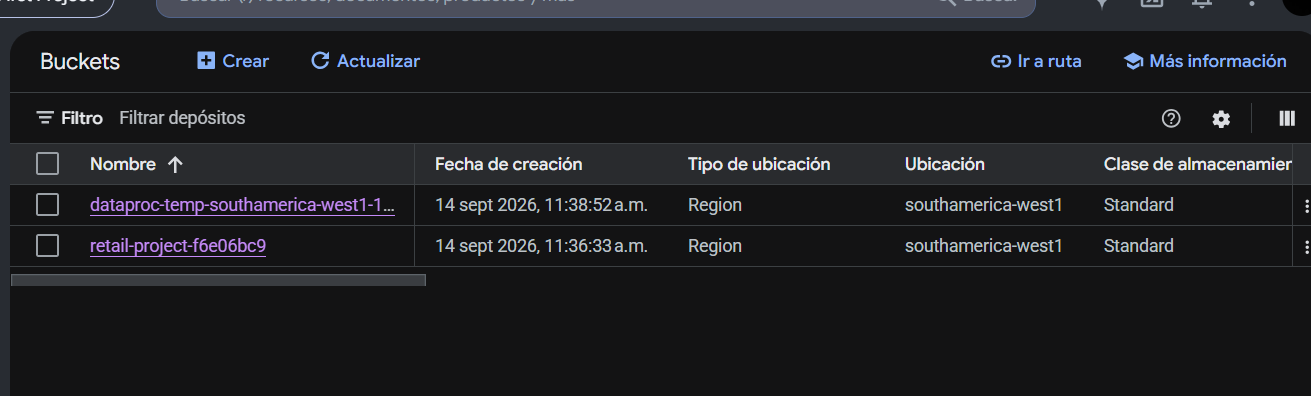
\includegraphics[width=0.85\textwidth]{../evidencia/bucket-lista.png}
    \caption{Bucket del proyecto en la lista de Cloud Storage}
    \label{fig:bucket-lista}
\end{figure}

Las Figuras \ref{fig:bucket-raw}, \ref{fig:bucket-input} y \ref{fig:bucket-output} muestran el contenido real de cada una de las tres carpetas.

\begin{figure}[h]
    \centering
    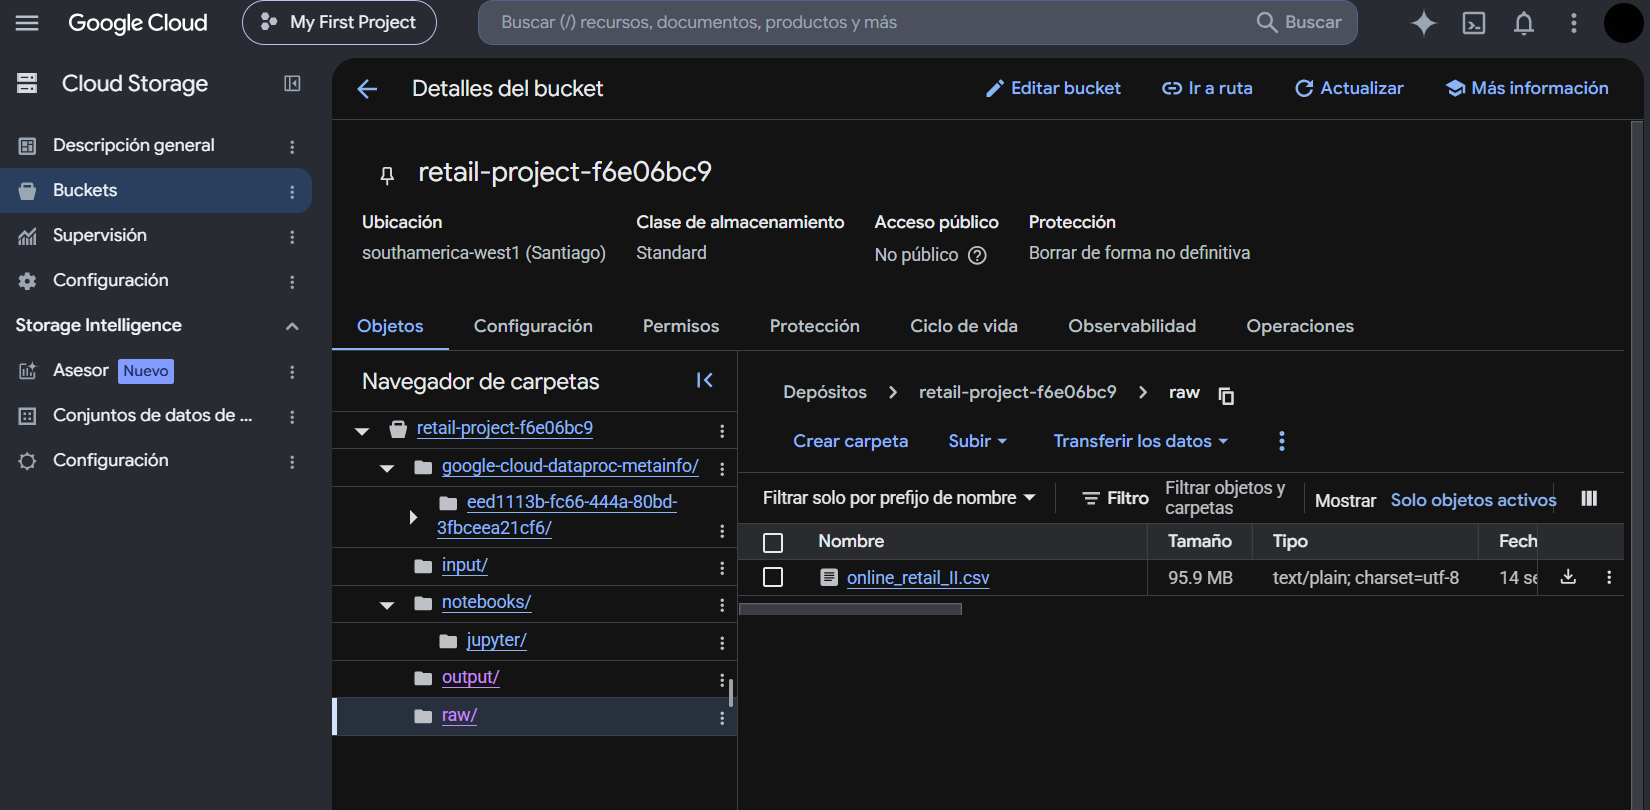
\includegraphics[width=0.85\textwidth]{../evidencia/bucket-raw.png}
    \caption{Carpeta \texttt{raw/}: el dataset original (\texttt{online\_retail\_II.csv}, 95.9 MB)}
    \label{fig:bucket-raw}
\end{figure}

\begin{figure}[h]
    \centering
    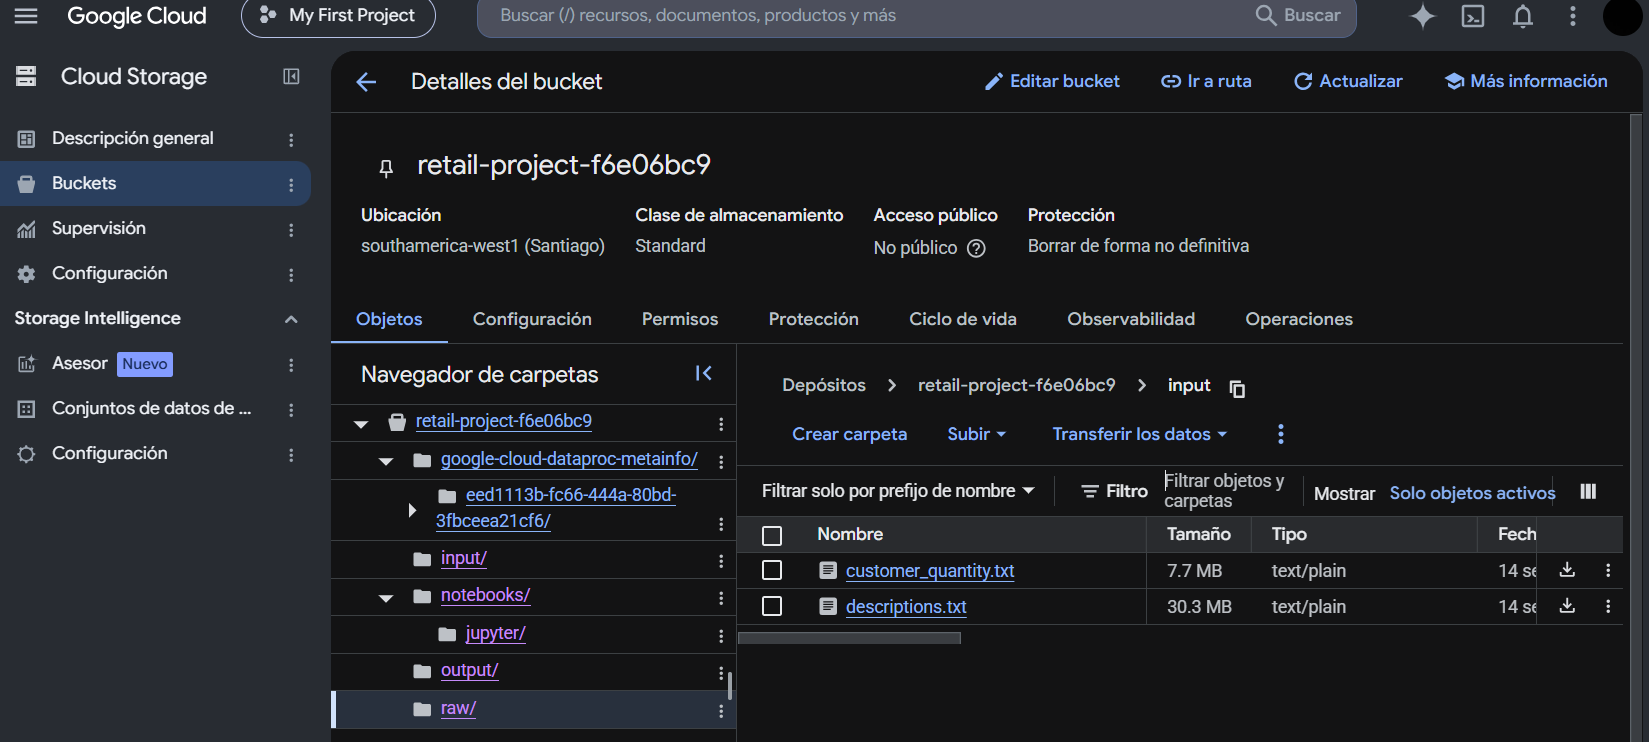
\includegraphics[width=0.85\textwidth]{../evidencia/bucket-input.png}
    \caption{Carpeta \texttt{input/}: archivos preparados para Hadoop MapReduce}
    \label{fig:bucket-input}
\end{figure}

\begin{figure}[h]
    \centering
    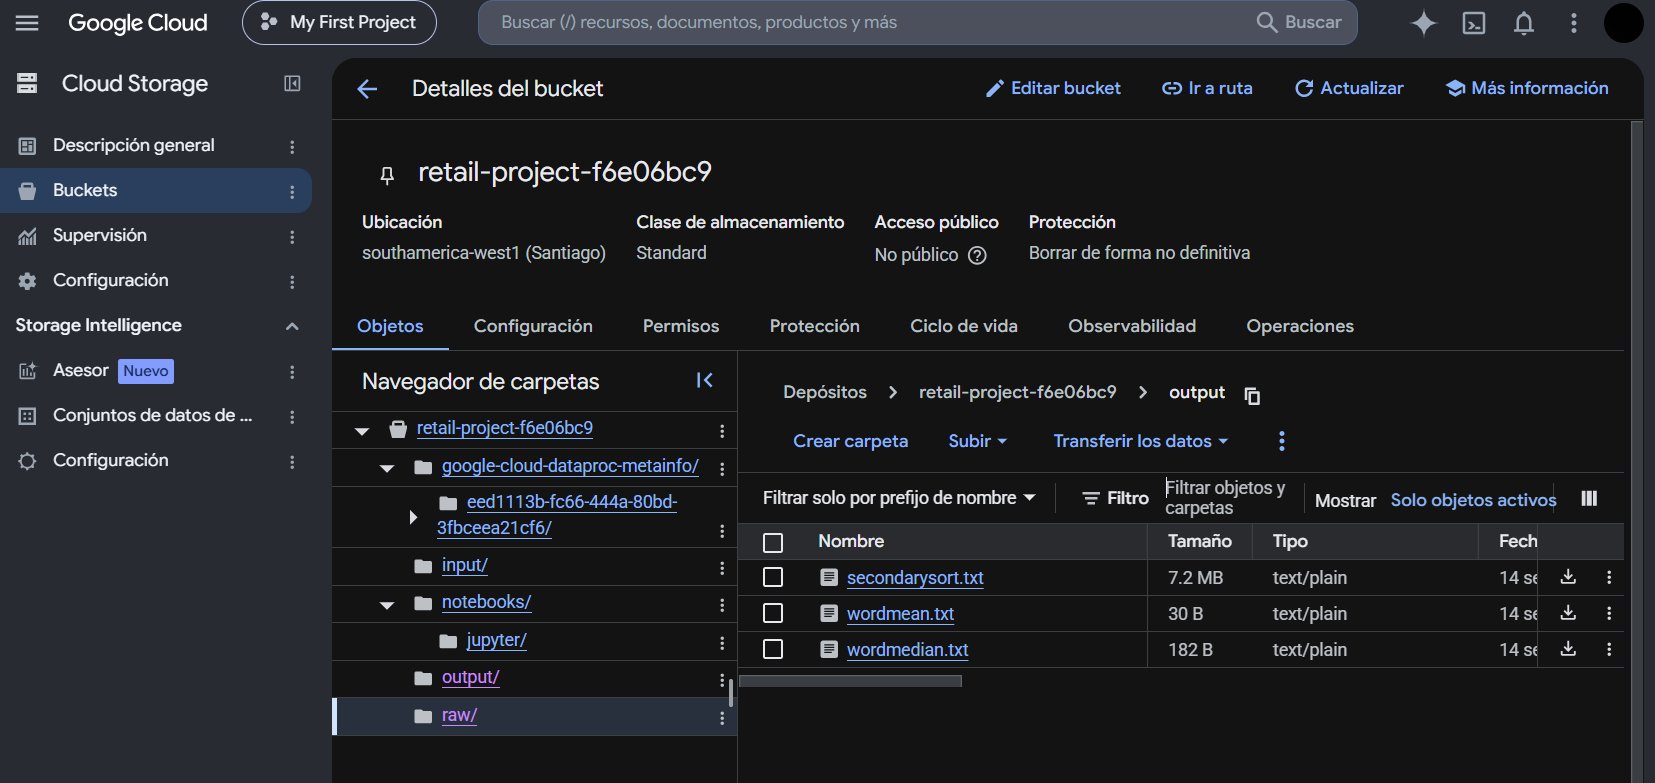
\includegraphics[width=0.85\textwidth]{../evidencia/bucket-output.png}
    \caption{Carpeta \texttt{output/}: resultados de los tres programas de Hadoop MapReduce}
    \label{fig:bucket-output}
\end{figure}

\subsubsection*{Justificación del uso de almacenamiento en la nube}

Se optó por Cloud Storage en vez de, por ejemplo, disco local del clúster, por tres razones concretas. Primero, Cloud Storage separa el cómputo del almacenamiento: los datos persisten en el bucket incluso si el clúster Dataproc se destruye, lo cual es clave porque el clúster se apaga y se vuelve a crear varias veces a lo largo del proyecto (y de hecho se apaga automáticamente todos los días como respaldo de costos, ver más abajo). Segundo, Dataproc integra de forma nativa un conector a Cloud Storage, por lo que tanto Spark como Hadoop MapReduce pueden leer y escribir directamente sobre \texttt{gs://} sin configuración adicional. Tercero, organizar el bucket en tres zonas (\texttt{raw/}, \texttt{input/}, \texttt{output/}) permite simular, con una sola herramienta, las etapas típicas de un data lake real: datos crudos, datos preparados, y resultados.

\subsection{Clúster Dataproc}

El clúster se aprovisionó en modo \emph{Standard}: 1 nodo master + 2 nodos worker, todos \texttt{n4-standard-2} (2 vCPU, 8 GB RAM) con disco \texttt{hyperdisk-balanced} de 100 GB. Dataproc administra de forma nativa Spark, Hadoop y HDFS sobre este clúster, con el conector a Cloud Storage ya configurado.

Por seguridad, el clúster no tiene IP pública (\texttt{internal\_ip\_only = true}): el acceso es exclusivamente por SSH vía IAP tunneling o por el Component Gateway (JupyterLab, Spark History Server), nunca por una IP directa. Para que el clúster tenga salida a internet (necesaria para instalar dependencias de Python o clonar el repositorio) sin exponer una IP pública, se agregó un Cloud NAT (Cloud Router + Cloud NAT), que permite tráfico saliente sin aceptar ninguna conexión entrante.

Como respaldo de costos, se configuró un job de Cloud Scheduler que apaga el clúster automáticamente todos los días a una hora fija, por si el equipo olvida apagarlo manualmente.

\subsubsection*{Evidencia}

\begin{figure}[h]
    \centering
    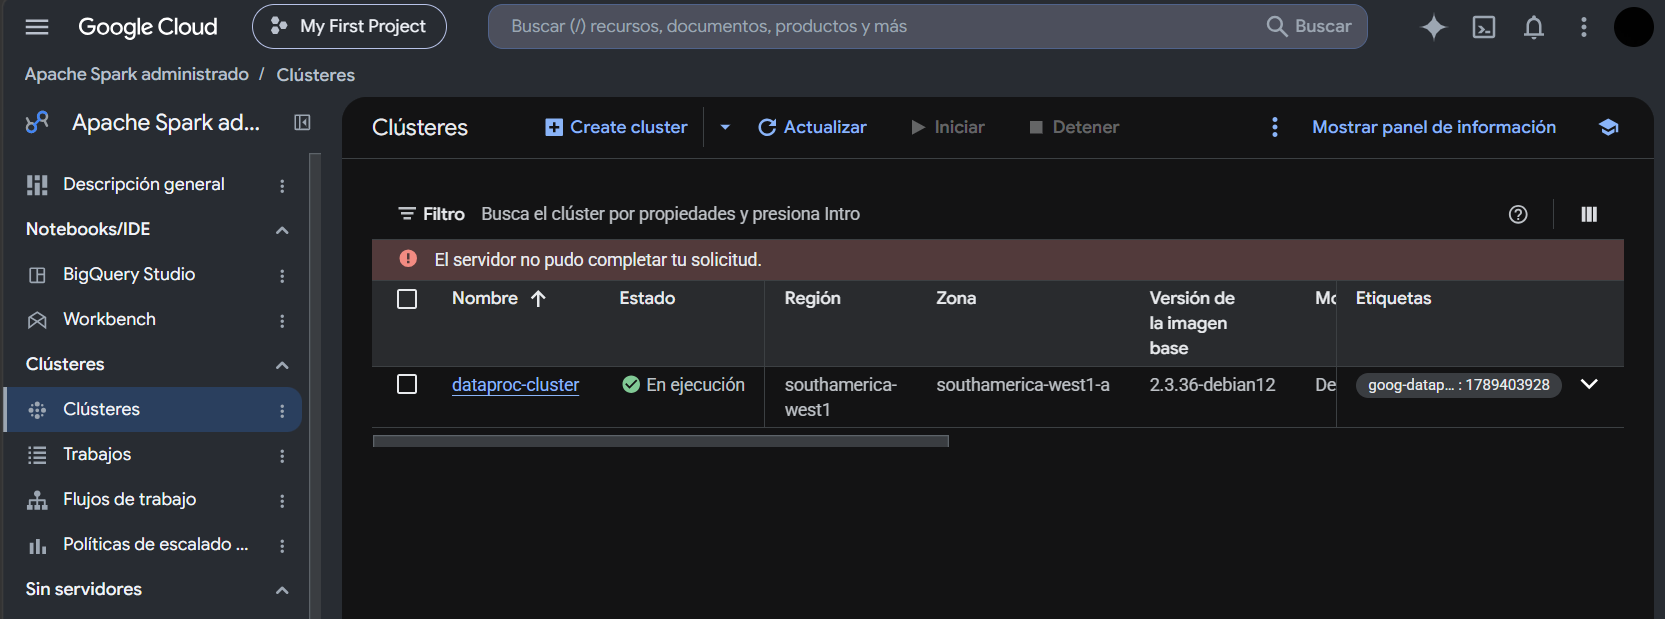
\includegraphics[width=0.85\textwidth]{../evidencia/cluster-running.png}
    \caption{Clúster \texttt{dataproc-cluster} en estado \emph{En ejecución}}
    \label{fig:cluster-running}
\end{figure}

\begin{figure}[h]
    \centering
    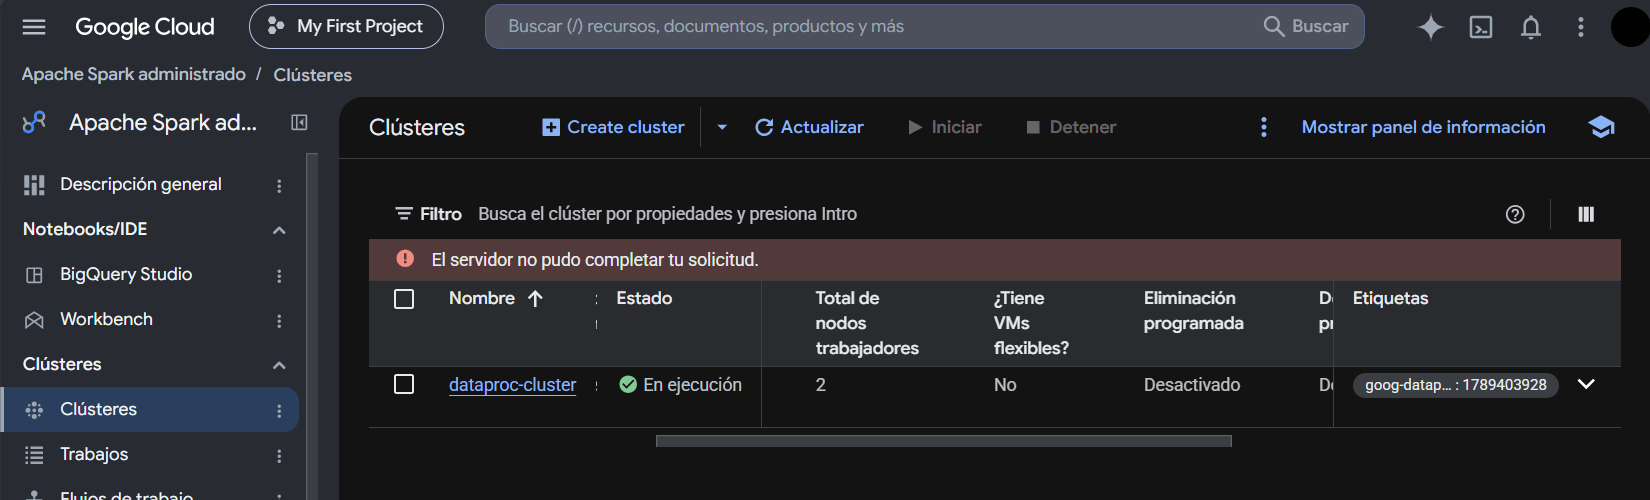
\includegraphics[width=0.85\textwidth]{../evidencia/cluster-workers.png}
    \caption{Detalle del clúster: 2 nodos trabajadores confirmados}
    \label{fig:cluster-workers}
\end{figure}

\subsection{Reproducibilidad con Terraform}

Toda la infraestructura descrita en esta sección —bucket, clúster, service account de apagado automático y job de Cloud Scheduler— está definida en \texttt{terraform/main.tf}. Cualquier integrante del equipo puede levantar una copia idéntica de esta infraestructura en su propio proyecto de GCP corriendo \texttt{terraform apply}, y destruirla por completo con \texttt{terraform destroy}, sin dejar recursos huérfanos ni pasos manuales pendientes.
